\documentclass{article}

% content/resources/templates/preamble.tex
\usepackage[margin=0.6in]{geometry}
\author{Milav Dabgar}
\usepackage{amsmath,amssymb,amsthm}
\usepackage{booktabs}
\usepackage{multirow}
\usepackage{xcolor}
\usepackage{tcolorbox}
\tcbuselibrary{breakable,skins}
\usepackage[colorlinks=true,linkcolor=blue]{hyperref}
\usepackage{titlesec}
\usepackage{enumitem}
\usepackage{tikz}
\usepackage{pgfplots}
\usepackage{circuitikz}
\usepackage[version=4]{mhchem}
\usepackage{longtable}
\usepackage{array}
\usepackage{float}
\usepackage{caption}
\usepackage{listings}

\lstset{
  basicstyle=\small\ttfamily,
  breaklines=true,
  breakatwhitespace=false,
  postbreak=\mbox{\textcolor{red}{$\hookrightarrow$}\space},
  float=false,
  numbers=left,
  numberstyle=\tiny\color{gray},
  numbersep=10pt,
  xleftmargin=2em,
  keywordstyle=\color{blue},
  commentstyle=\color{green!60!black},
  stringstyle=\color{purple},
  backgroundcolor=\color{gray!5},
  showstringspaces=false,
  tabsize=2,
  captionpos=b,
  keepspaces=true,
  columns=flexible
}

\pgfplotsset{compat=1.18}
\usetikzlibrary{shapes,arrows,positioning,calc,patterns,decorations.pathmorphing,decorations.markings,arrows.meta}

% Color scheme
\definecolor{headcolor}{RGB}{0,102,204}
\definecolor{keycolor}{RGB}{220,20,60}
\definecolor{solutioncolor}{RGB}{34,139,34}
\definecolor{mnemoniccolor}{RGB}{148,0,211}
\definecolor{codecolor}{RGB}{0,0,100}

% Spacing
\setlength{\parskip}{3pt}
\setlist[itemize]{nosep}
\setlist[enumerate]{nosep}

% Title formatting
\titleformat{\section}{\Large\bfseries\color{headcolor}}{\thesection}{1em}{}
\titleformat{\subsection}{\large\bfseries\color{headcolor}}{\thesubsection}{1em}{}

% Pandoc tightlist compatibility
\providecommand{\tightlist}{%
  \setlength{\itemsep}{0pt}\setlength{\parskip}{0pt}}

% Pandoc longtable compatibility
\newcounter{none}
\def\thenone{}


% content/resources/templates/english-boxes.tex

% Custom environments
\newtcolorbox{solutionbox}{
 breakable,
 enhanced,
 colback=solutioncolor!5!white,
 colframe=solutioncolor!75!black,
 fonttitle=\bfseries,
 title=Solution
}

\newtcolorbox{solutionboxnobreak}{
 colback=solutioncolor!5!white,
 colframe=solutioncolor!75!black,
 fonttitle=\bfseries,
 title=Solution
}

\newtcolorbox{keyformula}{
 breakable,
 enhanced,
 colback=keycolor!5!white,
 colframe=keycolor!75!black,
 fonttitle=\bfseries,
 title=Key Formula
}

\newtcolorbox{mnemonicboxenv}{
 breakable,
 enhanced,
 colback=mnemoniccolor!5!white,
 colframe=mnemoniccolor!75!black,
 fonttitle=\bfseries,
 title=Mnemonic
}

\newcommand{\mnemonicbox}[1]{%
  \begin{mnemonicboxenv}
    #1
  \end{mnemonicboxenv}
}


% Custom commands for GTU solutions
% This file defines semantic commands for consistent formatting

% Question command with automatic formatting
\newcommand{\question}[2]{%
  \section*{Question #1}%
  \textbf{#2}%
}

% OR question variant
\newcommand{\questionor}[2]{%
  \section*{Question #1 OR}%
  \textbf{#2}%
}

% Proper table environment with caption
\newenvironment{answertable}[1]{%
  \begin{table}[htbp]
  \centering
  \caption{#1}
}{%
  \end{table}
}

% Proper figure environment for diagrams
\newenvironment{answerdiagram}[1]{%
  \begin{figure}[htbp]
  \centering
  \caption{#1}
}{%
  \end{figure}
}

% Semantic markup for key terms
\newcommand{\keyword}[1]{\textbf{#1}}
\newcommand{\code}[1]{\texttt{#1}}
\newcommand{\classname}[1]{\texttt{#1}}
\newcommand{\methodname}[1]{\texttt{#1}}

% Proper quotation marks
\newcommand{\mnemonic}[1]{``#1''}


\title{Computer Networks \& Data Communication (4361101) - Summer 2025 Solution}
\date{May 08, 2025}

\begin{document}
\maketitle

\questionmarks{1(a)}{3}{State different DSL technology and discuss ADSL}

\begin{solutionbox}

\textbf{DSL Technology Types:}

\begin{table}[H]
\centering
\begin{tabulary}{\textwidth}{L L L}
\toprule
\textbf{DSL Type} & \textbf{Full Name} & \textbf{Speed} \\
\midrule
\textbf{ADSL} & Asymmetric DSL & 1-8 Mbps \\
\textbf{SDSL} & Symmetric DSL & 768 Kbps \\
\textbf{VDSL} & Very high DSL & 52 Mbps \\
\textbf{HDSL} & High bit-rate DSL & 1.5 Mbps \\
\bottomrule
\end{tabulary}
\caption{DSL Variants}
\end{table}

\textbf{ADSL Features:}
\begin{itemize}
    \item \textbf{Asymmetric}: Different upload/download speeds
    \item \textbf{Frequency Division}: Uses existing copper telephone lines
    \item \textbf{Download Speed}: Higher than upload speed
\end{itemize}

\end{solutionbox}

\begin{mnemonicbox}
\mnemonic{ADSL Downloads Faster}
\end{mnemonicbox}

\questionmarks{1(b)}{4}{Describe the network classification of based on Architecture.}

\begin{solutionbox}

\textbf{Network Architecture Classification:}

\begin{table}[H]
\centering
\begin{tabulary}{\textwidth}{L L L}
\toprule
\textbf{Architecture} & \textbf{Description} & \textbf{Features} \\
\midrule
\textbf{Peer-to-Peer} & All nodes equal & No central server \\
\textbf{Client-Server} & Centralized model & Dedicated server \\
\bottomrule
\end{tabulary}
\caption{Network Architectures}
\end{table}

\textbf{Client-Server Advantages:}
\begin{itemize}
    \item \textbf{Centralized Control}: Easy management and security
    \item \textbf{Resource Sharing}: Efficient utilization of resources
    \item \textbf{Scalability}: Can handle more users effectively
    \item \textbf{Data Security}: Better backup and recovery
\end{itemize}

\textbf{P2P Characteristics:}
\begin{itemize}
    \item \textbf{Decentralized}: No single point of failure
    \item \textbf{Cost Effective}: No need for dedicated server
\end{itemize}

\end{solutionbox}

\begin{mnemonicbox}
\mnemonic{Client Serves Better}
\end{mnemonicbox}

\questionmarks{1(c)}{7}{Draw the diagram of OSI Model and explain in detail with all layers.}

\begin{solutionbox}

\begin{figure}[H]
\centering
\begin{tikzpicture}[node distance=0.8cm, auto]
    \node (app) [gtu block, minimum width=5cm] {7. Application Layer};
    \node (pres) [gtu block, below=of app, minimum width=5cm] {6. Presentation Layer};
    \node (sess) [gtu block, below=of pres, minimum width=5cm] {5. Session Layer};
    \node (trans) [gtu block, below=of sess, minimum width=5cm] {4. Transport Layer};
    \node (net) [gtu block, below=of trans, minimum width=5cm] {3. Network Layer};
    \node (dl) [gtu block, below=of net, minimum width=5cm] {2. Data Link Layer};
    \node (phy) [gtu block, below=of dl, minimum width=5cm] {1. Physical Layer};
    
    \draw[gtu arrow] (app) -- (pres);
    \draw[gtu arrow] (pres) -- (sess);
    \draw[gtu arrow] (sess) -- (trans);
    \draw[gtu arrow] (trans) -- (net);
    \draw[gtu arrow] (net) -- (dl);
    \draw[gtu arrow] (dl) -- (phy);
\end{tikzpicture}
\caption{OSI Reference Model}
\end{figure}

\textbf{OSI Layer Functions:}

\begin{table}[H]
\centering
\begin{tabulary}{\textwidth}{L L L}
\toprule
\textbf{Layer} & \textbf{Function} & \textbf{Examples} \\
\midrule
\textbf{Application} & User interface & HTTP, FTP, SMTP \\
\textbf{Presentation} & Data formatting & Encryption, Compression \\
\textbf{Session} & Session management & NetBIOS, RPC \\
\textbf{Transport} & End-to-end delivery & TCP, UDP \\
\textbf{Network} & Routing & IP, ICMP \\
\textbf{Data Link} & Frame delivery & Ethernet, PPP \\
\textbf{Physical} & Bit transmission & Cables, Signals \\
\bottomrule
\end{tabulary}
\caption{Layer Functions}
\end{table}

\textbf{Key Features:}
\begin{itemize}
    \item \textbf{Layered Approach}: Each layer serves specific function
    \item \textbf{Standardization}: Universal communication model
    \item \textbf{Troubleshooting}: Easy to identify network problems
\end{itemize}

\end{solutionbox}

\begin{mnemonicbox}
\mnemonic{All People Seem To Need Data Processing}
\end{mnemonicbox}

\questionmarks{1(c OR)}{7}{Draw the diagram of TCP/IP protocol suite and explain the functions of Application Layer, Transport Layer and Network Layer in detail.}

\begin{solutionbox}

\begin{figure}[H]
\centering
\begin{tikzpicture}[node distance=1cm, auto]
    \node (app) [gtu block, minimum width=6cm] {Application Layer\\(HTTP, FTP, SMTP, DNS)};
    \node (trans) [gtu block, below=of app, minimum width=6cm] {Transport Layer\\(TCP, UDP)};
    \node (net) [gtu block, below=of trans, minimum width=6cm] {Network Layer\\(IP, ICMP, ARP)};
    \node (link) [gtu block, below=of net, minimum width=6cm] {Data Link Layer\\(Ethernet, Wi-Fi)};
    
    \draw[gtu arrow] (app) -- (trans);
    \draw[gtu arrow] (trans) -- (net);
    \draw[gtu arrow] (net) -- (link);
\end{tikzpicture}
\caption{TCP/IP Protocol Suite}
\end{figure}

\textbf{Layer Functions:}

\begin{table}[H]
\centering
\begin{tabulary}{\textwidth}{L L L}
\toprule
\textbf{Layer} & \textbf{Primary Function} & \textbf{Protocols} \\
\midrule
\textbf{Application} & User services & HTTP, FTP, SMTP \\
\textbf{Transport} & End-to-end delivery & TCP, UDP \\
\textbf{Network} & Routing packets & IP, ICMP \\
\bottomrule
\end{tabulary}
\caption{TCP/IP Layers}
\end{table}

\textbf{Application Layer Functions:}
\begin{itemize}
    \item \textbf{Web Services}: HTTP for web browsing
    \item \textbf{File Transfer}: FTP for file sharing
    \item \textbf{Email}: SMTP for mail delivery
\end{itemize}

\textbf{Transport Layer Functions:}
\begin{itemize}
    \item \textbf{Reliable Delivery}: TCP ensures data integrity
    \item \textbf{Unreliable Delivery}: UDP for fast transmission
    \item \textbf{Port Numbers}: Identify specific applications
\end{itemize}

\textbf{Network Layer Functions:}
\begin{itemize}
    \item \textbf{Logical Addressing}: IP addresses for devices
    \item \textbf{Routing}: Best path selection for packets
    \item \textbf{Fragmentation}: Breaking large packets
\end{itemize}

\end{solutionbox}

\begin{mnemonicbox}
\mnemonic{Applications Transport Networks}
\end{mnemonicbox}

\questionmarks{2(a)}{3}{Explain WWW.}

\begin{solutionbox}

\textbf{World Wide Web (WWW):}

\begin{table}[H]
\centering
\begin{tabulary}{\textwidth}{L L}
\toprule
\textbf{Component} & \textbf{Description} \\
\midrule
\textbf{Web Browser} & Client software (e.g., Chrome) \\
\textbf{Web Server} & Hosts websites (e.g., Apache) \\
\textbf{HTTP} & Communication protocol \\
\textbf{URL} & Web address \\
\bottomrule
\end{tabulary}
\caption{WWW Components}
\end{table}

\textbf{WWW Features:}
\begin{itemize}
    \item \textbf{Hypertext}: Linked documents using HTML
    \item \textbf{Client-Server Model}: Browser requests, server responds
    \item \textbf{Universal Access}: Platform independent
\end{itemize}

\end{solutionbox}

\begin{mnemonicbox}
\mnemonic{Web Works Worldwide}
\end{mnemonicbox}

\questionmarks{2(b)}{4}{Explain FDDI and CDDI.}

\begin{solutionbox}

\textbf{FDDI vs CDDI Comparison:}

\begin{table}[H]
\centering
\begin{tabulary}{\textwidth}{L L L}
\toprule
\textbf{Feature} & \textbf{FDDI} & \textbf{CDDI} \\
\midrule
\textbf{Medium} & Fiber optic & Copper wire \\
\textbf{Speed} & 100 Mbps & 100 Mbps \\
\textbf{Distance} & 200 km & 100 meters \\
\textbf{Cost} & High & Low \\
\bottomrule
\end{tabulary}
\caption{FDDI vs CDDI}
\end{table}

\textbf{FDDI Features:}
\begin{itemize}
    \item \textbf{Dual Ring Topology}: Primary and secondary rings
    \item \textbf{Token Passing}: Access control mechanism
    \item \textbf{Fault Tolerance}: Self-healing capability
\end{itemize}

\textbf{CDDI Features:}
\begin{itemize}
    \item \textbf{Copper Based}: Uses twisted pair cables
    \item \textbf{Cost Effective}: Cheaper than fiber
    \item \textbf{Limited Distance}: Shorter transmission range
\end{itemize}

\end{solutionbox}

\begin{mnemonicbox}
\mnemonic{Fiber Fast, Copper Cheap}
\end{mnemonicbox}

\questionmarks{2(c)}{7}{Describe Network management system with functions of OS, CLI, Administrative functions, interfaces.}

\begin{solutionbox}

\begin{figure}[H]
\centering
\begin{tikzpicture}[node distance=1.5cm, auto]
    \node (nms) [gtu block, minimum width=4cm] {Network Management System};
    \node (os) [gtu block, below left=of nms, xshift=-1cm] {Operating System};
    \node (cli) [gtu block, below right=of nms, xshift=1cm] {CLI Interface};
    \node (admin) [gtu block, below=of os] {Administrative Functions};
    \node (gui) [gtu block, below=of cli] {GUI Interfaces};
    
    \draw[gtu arrow] (nms) -- (os);
    \draw[gtu arrow] (nms) -- (cli);
    \draw[gtu arrow] (nms) -- (admin);
    \draw[gtu arrow] (nms) -- (gui);
    
    \node [below=0.2cm of os] {\small Resource Management};
    \node [below=0.2cm of cli] {\small Command Line};
    \node [below=0.2cm of admin] {\small User Management};
    \node [below=0.2cm of gui] {\small Graphical Interface};
\end{tikzpicture}
\caption{Network Management System}
\end{figure}

\textbf{Network Management Components:}

\begin{table}[H]
\centering
\begin{tabulary}{\textwidth}{L L L}
\toprule
\textbf{Component} & \textbf{Function} & \textbf{Examples} \\
\midrule
\textbf{OS Functions} & Resource management & Process, memory, file management \\
\textbf{CLI} & Command interface & Terminal, console commands \\
\textbf{Admin Functions} & System control & User accounts, security \\
\textbf{Interfaces} & User interaction & GUI, web interface \\
\bottomrule
\end{tabulary}
\caption{System Functions}
\end{table}

\textbf{Operating System Functions:}
\begin{itemize}
    \item \textbf{Process Management}: Controlling running applications
    \item \textbf{Memory Management}: Allocating system resources
    \item \textbf{File System}: Organizing and storing data
\end{itemize}

\textbf{CLI Functions:}
\begin{itemize}
    \item \textbf{Direct Commands}: Text-based control
    \item \textbf{Scripting}: Automation of tasks
    \item \textbf{Remote Access}: SSH, Telnet connections
\end{itemize}

\textbf{Administrative Functions:}
\begin{itemize}
    \item \textbf{User Management}: Creating, modifying user accounts
    \item \textbf{Security Policies}: Access control, permissions
    \item \textbf{System Monitoring}: Tracking performance
\end{itemize}

\end{solutionbox}

\begin{mnemonicbox}
\mnemonic{OS CLI Admin Interfaces}
\end{mnemonicbox}

\questionmarks{2(a OR)}{3}{Compare connection-oriented protocol and connectionless protocol.}

\begin{solutionbox}

\textbf{Protocol Comparison:}

\begin{table}[H]
\centering
\begin{tabulary}{\textwidth}{L L L}
\toprule
\textbf{Feature} & \textbf{Connection-Oriented} & \textbf{Connectionless} \\
\midrule
\textbf{Setup} & Required & Not required \\
\textbf{Reliability} & High & Low \\
\textbf{Speed} & Slower & Faster \\
\textbf{Example} & TCP & UDP \\
\bottomrule
\end{tabulary}
\caption{Connection vs Connectionless}
\end{table}

\textbf{Connection-Oriented Features:}
\begin{itemize}
    \item \textbf{Three-way Handshake}: Establishes connection before transfer
    \item \textbf{Reliable Delivery}: Guarantees packet delivery and order
\end{itemize}

\textbf{Connectionless Features:}
\begin{itemize}
    \item \textbf{No Setup}: Sends data immediately
    \item \textbf{Best Effort}: No guarantee of delivery
\end{itemize}

\end{solutionbox}

\begin{mnemonicbox}
\mnemonic{TCP Connects, UDP Delivers}
\end{mnemonicbox}

\questionmarks{2(b OR)}{4}{Explain Network device Repeater.}

\begin{solutionbox}

\textbf{Repeater Functions:}

\begin{table}[H]
\centering
\begin{tabulary}{\textwidth}{L L}
\toprule
\textbf{Function} & \textbf{Description} \\
\midrule
\textbf{Signal Amplification} & Boosts weak signals \\
\textbf{Range Extension} & Increases network distance \\
\textbf{Noise Reduction} & Cleans signal quality \\
\bottomrule
\end{tabulary}
\caption{Repeater Functions}
\end{table}

\begin{figure}[H]
\centering
\begin{tikzpicture}[node distance=2.5cm, auto]
    \node (weak) [gtu input] {Weak Signal};
    \node (rep) [gtu process, right=of weak] {REPEATER\\(Amplify)};
    \node (strong) [gtu input, right=of rep] {Strong Signal};
    
    \draw[gtu arrow] (weak) -- node[midway, above] {Noisy} (rep);
    \draw[gtu arrow] (rep) -- node[midway, above] {Clean} (strong);
\end{tikzpicture}
\caption{Repeater Operation}
\end{figure}

\textbf{Repeater Characteristics:}
\begin{itemize}
    \item \textbf{Physical Layer Device}: Operates at Layer 1
    \item \textbf{Bit-by-Bit}: Regenerates digital signals
    \item \textbf{No Intelligence}: Cannot filter or route data
\end{itemize}

\end{solutionbox}

\begin{mnemonicbox}
\mnemonic{Repeater Regenerates Signals}
\end{mnemonicbox}

\questionmarks{2(c OR)}{7}{Differentiate between Router, Hub and Switch.}

\begin{solutionbox}

\textbf{Network Device Comparison:}

\begin{table}[H]
\centering
\begin{tabulary}{\textwidth}{L L L L}
\toprule
\textbf{Feature} & \textbf{Hub} & \textbf{Switch} & \textbf{Router} \\
\midrule
\textbf{OSI Layer} & Physical (1) & Data Link (2) & Network (3) \\
\textbf{Collision Domain} & Single & Multiple & Multiple \\
\textbf{Broadcast Domain} & Single & Single & Multiple \\
\textbf{Intelligence} & None & Learn MAC & IP Routing \\
\textbf{Full Duplex} & No & Yes & Yes \\
\bottomrule
\end{tabulary}
\caption{Hub vs Switch vs Router}
\end{table}

\begin{figure}[H]
\centering
\begin{tikzpicture}[node distance=1.5cm, auto]
    \node (dev) [gtu block, minimum width=4cm] {Network Devices};
    \node (hub) [gtu block, below left=of dev, xshift=-2cm] {Hub\\(Layer 1)};
    \node (sw) [gtu block, below=of dev] {Switch\\(Layer 2)};
    \node (rtr) [gtu block, below right=of dev, xshift=2cm] {Router\\(Layer 3)};
    
    \draw[gtu arrow] (dev) -- (hub);
    \draw[gtu arrow] (dev) -- (sw);
    \draw[gtu arrow] (dev) -- (rtr);
    
    \node [below=0.2cm of hub, align=center, font=\footnotesize] {Shared\\Bandwidth};
    \node [below=0.2cm of sw, align=center, font=\footnotesize] {Dedicated\\Bandwidth};
    \node [below=0.2cm of rtr, align=center, font=\footnotesize] {Inter-network\\Connection};
\end{tikzpicture}
\caption{Network Devices Classification}
\end{figure}

\textbf{Hub Characteristics:}
\begin{itemize}
    \item \textbf{Shared Medium}: All ports share bandwidth
    \item \textbf{Half Duplex}: Cannot send and receive simultaneously
    \item \textbf{Collision Prone}: Single collision domain
\end{itemize}

\textbf{Switch Characteristics:}
\begin{itemize}
    \item \textbf{MAC Address Table}: Learns device locations
    \item \textbf{Full Duplex}: Simultaneous send/receive
    \item \textbf{VLAN Support}: Virtual network segmentation
\end{itemize}

\textbf{Router Characteristics:}
\begin{itemize}
    \item \textbf{IP Routing}: Forwards packets between networks
    \item \textbf{Routing Table}: Maintains network topology
    \item \textbf{NAT Support}: Network Address Translation
\end{itemize}

\end{solutionbox}

\begin{mnemonicbox}
\mnemonic{Hub Shares, Switch Switches, Router Routes}
\end{mnemonicbox}

\questionmarks{3(a)}{3}{Draw neat diagram of UTP, Coaxial and Fiber optic cable}

\begin{solutionbox}

\begin{figure}[H]
\centering
\begin{center}
\textbf{1. UTP Cable}
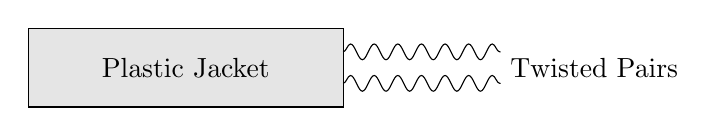
\begin{tikzpicture}
    % Outer Jacket
    \draw[fill=gray!20] (0,0) rectangle (4,1);
    \node at (2, 0.5) {Plastic Jacket};
    % Twisted Pairs (Simulated)
    \draw[decorate, decoration={snake, amplitude=1mm, segment length=3mm}] (4, 0.7) -- (6, 0.7);
    \draw[decorate, decoration={snake, amplitude=1mm, segment length=3mm}] (4, 0.3) -- (6, 0.3);
    \node[right] at (6, 0.5) {Twisted Pairs};
\end{tikzpicture}

\vspace{0.5cm}
\textbf{2. Coaxial Cable}
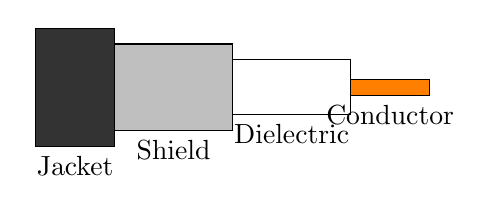
\begin{tikzpicture}
    % Layers
    \draw[fill=black!80] (0,0) rectangle (1,1.5); % Jacket
    \draw[fill=gray!50] (1,0.2) rectangle (2.5,1.3); % Shield
    \draw[fill=white] (2.5,0.4) rectangle (4,1.1); % Dielectric
    \draw[fill=orange] (4,0.65) rectangle (5,0.85); % Conductor
    
    \node[below] at (0.5,0) {Jacket};
    \node[below] at (1.75,0.2) {Shield};
    \node[below] at (3.25,0.4) {Dielectric};
    \node[below] at (4.5,0.65) {Conductor};
\end{tikzpicture}

\vspace{0.5cm}
\textbf{3. Fiber Optic Cable}
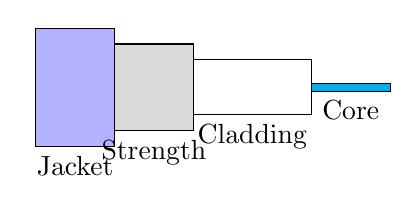
\begin{tikzpicture}
    % Layers
    \draw[fill=blue!30] (0,0) rectangle (1,1.5); % Jacket
    \draw[fill=gray!30] (1,0.2) rectangle (2,1.3); % Strength
    \draw[fill=white] (2,0.4) rectangle (3.5,1.1); % Cladding
    \draw[fill=cyan] (3.5,0.7) rectangle (4.5,0.8); % Core
    
    \node[below] at (0.5,0) {Jacket};
    \node[below] at (1.5,0.2) {Strength};
    \node[below] at (2.75,0.4) {Cladding};
    \node[below] at (4,0.7) {Core};
\end{tikzpicture}
\end{center}
\caption{Transmission Media Cables}
\end{figure}

\textbf{Cable Characteristics:}

\begin{table}[H]
\centering
\begin{tabulary}{\textwidth}{L L L}
\toprule
\textbf{Cable Type} & \textbf{Core Material} & \textbf{Bandwidth} \\
\midrule
\textbf{UTP} & Copper wire & 100 MHz \\
\textbf{Coaxial} & Copper conductor & 1 GHz \\
\textbf{Fiber Optic} & Glass/Plastic & Very high \\
\bottomrule
\end{tabulary}
\caption{Cable Comparison}
\end{table}

\end{solutionbox}

\begin{mnemonicbox}
\mnemonic{Twisted Copper Glass}
\end{mnemonicbox}

\questionmarks{3(b)}{4}{Differentiate switching circuit and packet switching circuit.}

\begin{solutionbox}

\textbf{Switching Methods Comparison:}

\begin{table}[H]
\centering
\begin{tabulary}{\textwidth}{L L L}
\toprule
\textbf{Feature} & \textbf{Circuit Switching} & \textbf{Packet Switching} \\
\midrule
\textbf{Path} & Dedicated & Shared \\
\textbf{Setup Time} & Required & Not required \\
\textbf{Bandwidth} & Fixed & Variable \\
\textbf{Example} & Telephone & Internet \\
\bottomrule
\end{tabulary}
\caption{Circuit vs Packet Switching}
\end{table}

\textbf{Circuit Switching Features:}
\begin{itemize}
    \item \textbf{Dedicated Path}: Exclusive connection between communicating parties
    \item \textbf{Constant Bandwidth}: Fixed data rate throughout communication
    \item \textbf{Setup Phase}: Connection established before data transfer
\end{itemize}

\textbf{Packet Switching Features:}
\begin{itemize}
    \item \textbf{Store and Forward}: Packets stored at intermediate nodes
    \item \textbf{Dynamic Routing}: Different paths for different packets
    \item \textbf{Resource Sharing}: Multiple users share network resources
\end{itemize}

\end{solutionbox}

\begin{mnemonicbox}
\mnemonic{Circuit Connects, Packet Shares}
\end{mnemonicbox}

\questionmarks{3(c)}{7}{Describe unguided media and guided media.}

\begin{solutionbox}

\begin{figure}[H]
\centering
\begin{tikzpicture}[node distance=1cm, auto]
    \node (media) [gtu block] {Transmission Media};
    \node (guided) [gtu block, below left=of media, xshift=-2cm] {Guided Media};
    \node (unguided) [gtu block, below right=of media, xshift=2cm] {Unguided Media};
    
    \node (tp) [gtu block, below=of guided, xshift=-1.5cm, font=\footnotesize] {Twisted Pair};
    \node (coax) [gtu block, right=0.2cm of tp, font=\footnotesize] {Coaxial};
    \node (fiber) [gtu block, right=0.2cm of coax, font=\footnotesize] {Fiber Optic};
    
    \node (radio) [gtu block, below=of unguided, xshift=-1.5cm, font=\footnotesize] {Radio};
    \node (micro) [gtu block, right=0.2cm of radio, font=\footnotesize] {Microwave};
    \node (ir) [gtu block, right=0.2cm of micro, font=\footnotesize] {Infrared};
    
    \draw[gtu arrow] (media) -- (guided);
    \draw[gtu arrow] (media) -- (unguided);
    \draw[gtu arrow] (guided) -- (tp);
    \draw[gtu arrow] (guided) -- (coax);
    \draw[gtu arrow] (guided) -- (fiber);
    \draw[gtu arrow] (unguided) -- (radio);
    \draw[gtu arrow] (unguided) -- (micro);
    \draw[gtu arrow] (unguided) -- (ir);
\end{tikzpicture}
\caption{Transmission Media Classification}
\end{figure}

\textbf{Guided Media Characteristics:}

\begin{table}[H]
\centering
\begin{tabulary}{\textwidth}{L L L L}
\toprule
\textbf{Type} & \textbf{Material} & \textbf{Distance} & \textbf{Cost} \\
\midrule
\textbf{Twisted Pair} & Copper & 100m & Low \\
\textbf{Coaxial} & Copper + Shield & 500m & Medium \\
\textbf{Fiber Optic} & Glass & 2km+ & High \\
\bottomrule
\end{tabulary}
\caption{Guided Media}
\end{table}

\textbf{Unguided Media Characteristics:}

\begin{table}[H]
\centering
\begin{tabulary}{\textwidth}{L L L L}
\toprule
\textbf{Type} & \textbf{Frequency} & \textbf{Range} & \textbf{Application} \\
\midrule
\textbf{Radio Waves} & 3KHz-1GHz & Long & AM/FM Radio \\
\textbf{Microwaves} & 1GHz-300GHz & Line of sight & Satellite \\
\textbf{Infrared} & 300GHz-400THz & Short & Remote control \\
\bottomrule
\end{tabulary}
\caption{Unguided Media}
\end{table}

\end{solutionbox}

\begin{mnemonicbox}
\mnemonic{Guided Wires, Unguided Airs}
\end{mnemonicbox}

\questionmarks{3(a OR)}{3}{Discuss various connectors used in Computer Networks.}

\begin{solutionbox}

\textbf{Network Connectors:}

\begin{table}[H]
\centering
\begin{tabulary}{\textwidth}{L L L}
\toprule
\textbf{Connector} & \textbf{Cable Type} & \textbf{Application} \\
\midrule
\textbf{RJ-45} & UTP/STP & Ethernet \\
\textbf{BNC} & Coaxial & Legacy networks \\
\textbf{SC/ST} & Fiber optic & High-speed networks \\
\bottomrule
\end{tabulary}
\caption{Connectors}
\end{table}

\textbf{Connector Features:}
\begin{itemize}
    \item \textbf{RJ-45}: 8-pin modular connector for twisted pair
    \item \textbf{BNC}: Bayonet connector for coaxial cables
    \item \textbf{SC/ST}: Push-pull and twist-lock fiber connectors
\end{itemize}

\end{solutionbox}

\begin{mnemonicbox}
\mnemonic{RJ BNC Fiber Connect}
\end{mnemonicbox}

\questionmarks{3(b OR)}{4}{Explain IP addressing scheme with examples.}

\begin{solutionbox}

\textbf{IP Address Classes:}

\begin{table}[H]
\centering
\begin{tabulary}{\textwidth}{L L L L}
\toprule
\textbf{Class} & \textbf{Range} & \textbf{Default Mask} & \textbf{Example} \\
\midrule
\textbf{A} & 1-126 & /8 & 10.0.0.1 \\
\textbf{B} & 128-191 & /16 & 172.16.0.1 \\
\textbf{C} & 192-223 & /24 & 192.168.1.1 \\
\bottomrule
\end{tabulary}
\caption{IP Classes}
\end{table}

\textbf{IP Address Structure:}
\begin{itemize}
    \item \textbf{Network Part}: Identifies the network
    \item \textbf{Host Part}: Identifies the device
    \item \textbf{Subnet Mask}: Separates network and host portions
\end{itemize}

\textbf{Special Addresses:}
\begin{itemize}
    \item \textbf{Loopback}: 127.0.0.1 (localhost)
    \item \textbf{Private}: 10.x.x.x, 172.16.x.x, 192.168.x.x
    \item \textbf{Broadcast}: All host bits set to 1
\end{itemize}

\textbf{Example Calculation:}
\code{IP: 192.168.1.100/24}
\begin{itemize}
    \item Network: 192.168.1.0
    \item Broadcast: 192.168.1.255
\end{itemize}

\end{solutionbox}

\begin{mnemonicbox}
\mnemonic{A Big Class Networks}
\end{mnemonicbox}

\questionmarks{3(c OR)}{7}{Differentiate between IPv4 and IPv6.}

\begin{solutionbox}

\textbf{IPv4 vs IPv6 Comparison:}

\begin{table}[H]
\centering
\begin{tabulary}{\textwidth}{L L L}
\toprule
\textbf{Feature} & \textbf{IPv4} & \textbf{IPv6} \\
\midrule
\textbf{Address Length} & 32 bits & 128 bits \\
\textbf{Address Format} & Decimal & Hexadecimal \\
\textbf{Address Space} & 4.3 billion & 340 undecillion \\
\textbf{Header Size} & 20-60 bytes & 40 bytes \\
\textbf{Fragmentation} & Router/Host & Host only \\
\textbf{Security} & Optional & Built-in \\
\bottomrule
\end{tabulary}
\caption{IPv4 vs IPv6}
\end{table}

\textbf{IPv4 Characteristics:}
\begin{itemize}
    \item \textbf{Address Example}: 192.168.1.1
    \item \textbf{Dotted Decimal}: Four octets separated by dots
    \item \textbf{Classes}: A, B, C, D, E addressing scheme
    \item \textbf{NAT Required}: Due to address exhaustion
\end{itemize}

\textbf{IPv6 Characteristics:}
\begin{itemize}
    \item \textbf{Address Example}: 2001:0db8:85a3::8a2e:0370:7334
    \item \textbf{Colon Notation}: Eight groups of hexadecimal digits
    \item \textbf{No Classes}: Hierarchical addressing
    \item \textbf{Auto-configuration}: Stateless address configuration
\end{itemize}

\textbf{IPv6 Advantages:}
\begin{itemize}
    \item \textbf{Larger Address Space}: Eliminates address exhaustion
    \item \textbf{Simplified Header}: Improved processing efficiency
    \item \textbf{Built-in Security}: IPSec mandatory
    \item \textbf{Better QoS}: Flow labeling for traffic prioritization
\end{itemize}

\textbf{Migration Strategies:}
\begin{itemize}
    \item \textbf{Dual Stack}: Run both IPv4 and IPv6
    \item \textbf{Tunneling}: Encapsulate IPv6 in IPv4
    \item \textbf{Translation}: Convert between protocols
\end{itemize}

\end{solutionbox}

\begin{mnemonicbox}
\mnemonic{IPv6 Has More Addresses}
\end{mnemonicbox}

\questionmarks{4(a)}{3}{Explain File Transfer Protocol.}

\begin{solutionbox}

\textbf{FTP Characteristics:}

\begin{table}[H]
\centering
\begin{tabulary}{\textwidth}{L L}
\toprule
\textbf{Feature} & \textbf{Description} \\
\midrule
\textbf{Port Numbers} & 20 (data), 21 (control) \\
\textbf{Protocol} & TCP-based \\
\textbf{Authentication} & Username/password \\
\bottomrule
\end{tabulary}
\caption{FTP Basics}
\end{table}

\textbf{FTP Operations:}
\begin{itemize}
    \item \textbf{Upload}: PUT command to transfer files to server
    \item \textbf{Download}: GET command to retrieve files from server
    \item \textbf{Directory}: LIST command to show file listings
\end{itemize}

\end{solutionbox}

\begin{mnemonicbox}
\mnemonic{FTP Files Transfer Put Get}
\end{mnemonicbox}

\questionmarks{4(b)}{4}{Write short note on DNS.}

\begin{solutionbox}

\textbf{Domain Name System (DNS):}

\begin{table}[H]
\centering
\begin{tabulary}{\textwidth}{L L}
\toprule
\textbf{Component} & \textbf{Function} \\
\midrule
\textbf{DNS Server} & Resolves domain names \\
\textbf{DNS Cache} & Stores recent lookups \\
\textbf{DNS Records} & Maps names to addresses \\
\bottomrule
\end{tabulary}
\caption{DNS Components}
\end{table}

\textbf{DNS Hierarchy:}
\begin{itemize}
    \item \textbf{Root Domain}: Top-level (.)
    \item \textbf{Top-Level Domain}: .com, .org, .net
    \item \textbf{Second-Level Domain}: google.com
\end{itemize}

\end{solutionbox}

\begin{mnemonicbox}
\mnemonic{DNS Domain Names Servers}
\end{mnemonicbox}

\questionmarks{4(c)}{7}{Explain Electronic Mail.}

\begin{solutionbox}

\begin{figure}[H]
\centering
\begin{tikzpicture}[node distance=1.5cm, auto]
    \node (sender) [gtu block] {Email Client};
    \node (smtp) [gtu block, right=of sender] {SMTP Server};
    \node (internet) [gtu block, right=of smtp] {Internet};
    \node (rec_smtp) [gtu block, right=of internet] {Recipient SMTP};
    \node (pop) [gtu block, below=of rec_smtp] {POP3/IMAP};
    \node (receiver) [gtu block, left=of pop] {Recipient Client};
    
    \draw[gtu arrow] (sender) -- (smtp);
    \draw[gtu arrow] (smtp) -- (internet);
    \draw[gtu arrow] (internet) -- (rec_smtp);
    \draw[gtu arrow] (rec_smtp) -- (pop);
    \draw[gtu arrow] (pop) -- (receiver);
\end{tikzpicture}
\caption{Email Delivery System}
\end{figure}

\textbf{Email System Components:}

\begin{table}[H]
\centering
\begin{tabulary}{\textwidth}{L L L}
\toprule
\textbf{Component} & \textbf{Function} & \textbf{Protocol} \\
\midrule
\textbf{User Agent} & Email client & Outlook, Gmail \\
\textbf{Mail Server} & Store/forward & SMTP, POP3, IMAP \\
\textbf{Message Transfer} & Delivery & SMTP \\
\bottomrule
\end{tabulary}
\caption{Email Components}
\end{table}

\end{solutionbox}

\begin{mnemonicbox}
\mnemonic{SMTP Sends, POP3 Pulls, IMAP Integrates}
\end{mnemonicbox}

\questionmarks{4(a OR)}{3}{Explain Web browser.}

\begin{solutionbox}

\textbf{Web Browser Functions:}

\begin{table}[H]
\centering
\begin{tabulary}{\textwidth}{L L}
\toprule
\textbf{Function} & \textbf{Description} \\
\midrule
\textbf{HTTP Client} & Requests web pages \\
\textbf{HTML Renderer} & Displays web content \\
\textbf{JavaScript Engine} & Executes scripts \\
\bottomrule
\end{tabulary}
\caption{Browser Functions}
\end{table}

\end{solutionbox}

\begin{mnemonicbox}
\mnemonic{Browser Render Web Pages}
\end{mnemonicbox}

\questionmarks{4(b OR)}{4}{Explain Mail Protocols.}

\begin{solutionbox}

\textbf{Email Protocol Comparison:}

\begin{table}[H]
\centering
\begin{tabulary}{\textwidth}{L L L L}
\toprule
\textbf{Protocol} & \textbf{Type} & \textbf{Function} & \textbf{Port} \\
\midrule
\textbf{SMTP} & Outgoing & Send mail & 25 \\
\textbf{POP3} & Incoming & Download mail & 110 \\
\textbf{IMAP} & Incoming & Sync mail & 143 \\
\bottomrule
\end{tabulary}
\caption{Mail Protocols}
\end{table}

\textbf{SMTP Features:}
\begin{itemize}
    \item \textbf{Push Protocol}: Sender initiates transfer
    \item \textbf{Store and Forward}: Intermediate mail servers
    \item \textbf{Text-based}: ASCII command protocol
\end{itemize}

\textbf{POP3 Features:}
\begin{itemize}
    \item \textbf{Download and Delete}: Mail removed from server
    \item \textbf{Offline Access}: Local mail storage
\end{itemize}

\textbf{IMAP Features:}
\begin{itemize}
    \item \textbf{Server Storage}: Mail remains on server
    \item \textbf{Multi-device}: Access from multiple clients
\end{itemize}

\end{solutionbox}

\begin{mnemonicbox}
\mnemonic{SMTP Sends, POP3 Pulls, IMAP Integrates}
\end{mnemonicbox}

\questionmarks{4(c OR)}{7}{Describe TCP and UDP protocols.}

\begin{solutionbox}

\textbf{TCP vs UDP Comparison:}

\begin{table}[H]
\centering
\begin{tabulary}{\textwidth}{L L L}
\toprule
\textbf{Feature} & \textbf{TCP} & \textbf{UDP} \\
\midrule
\textbf{Connection} & Connection-oriented & Connectionless \\
\textbf{Reliability} & Reliable & Unreliable \\
\textbf{Speed} & Slower & Faster \\
\textbf{Header Size} & 20 bytes & 8 bytes \\
\textbf{Flow Control} & Yes & No \\
\textbf{Error Control} & Yes & No \\
\bottomrule
\end{tabulary}
\caption{TCP vs UDP}
\end{table}

\begin{figure}[H]
\centering
\begin{tikzpicture}[node distance=1.5cm, auto]
    \node (trans) [gtu block] {Transport Layer};
    \node (tcp) [gtu block, below left=of trans, xshift=-1cm] {TCP (Reliable)};
    \node (udp) [gtu block, below right=of trans, xshift=1cm] {UDP (Fast)};
    
    \node (tcp_apps) [gtu block, below=of tcp] {Web, Email, FTP};
    \node (udp_apps) [gtu block, below=of udp] {DNS, Streaming};
    
    \draw[gtu arrow] (trans) -- (tcp);
    \draw[gtu arrow] (trans) -- (udp);
    \draw[gtu arrow] (tcp) -- (tcp_apps);
    \draw[gtu arrow] (udp) -- (udp_apps);
\end{tikzpicture}
\caption{Transport Protocols}
\end{figure}

\textbf{TCP Features:}
\begin{itemize}
    \item \textbf{Three-way Handshake}: SYN, SYN-ACK, ACK
    \item \textbf{Sequence Numbers}: Ordered packet delivery
    \item \textbf{Acknowledgments}: Confirms packet receipt
\end{itemize}

\textbf{UDP Features:}
\begin{itemize}
    \item \textbf{Stateless}: No connection state maintained
    \item \textbf{Best Effort}: No delivery guarantee
    \item \textbf{Low Overhead}: Minimal header information
\end{itemize}

\end{solutionbox}

\begin{mnemonicbox}
\mnemonic{TCP Tries Carefully, UDP Unleashes Data}
\end{mnemonicbox}

\questionmarks{5(a)}{3}{Describe Network device Bridge.}

\begin{solutionbox}

\textbf{Bridge Characteristics:}

\begin{table}[H]
\centering
\begin{tabulary}{\textwidth}{L L}
\toprule
\textbf{Feature} & \textbf{Description} \\
\midrule
\textbf{OSI Layer} & Data Link (Layer 2) \\
\textbf{Function} & Segment collision domains \\
\textbf{Learning} & MAC address table \\
\bottomrule
\end{tabulary}
\caption{Bridge Functions}
\end{table}

\textbf{Bridge Operations:}
\begin{itemize}
    \item \textbf{Learning}: Records MAC addresses from frames
    \item \textbf{Filtering}: Forwards frames only when necessary
    \item \textbf{Forwarding}: Sends frames to appropriate segment
\end{itemize}

\end{solutionbox}

\begin{mnemonicbox}
\mnemonic{Bridge Breaks Collisions}
\end{mnemonicbox}

\questionmarks{5(b)}{4}{Explain Social issues and Hacking also discuss its precautions.}

\begin{solutionbox}

\textbf{Social Issues in Networks:}

\begin{table}[H]
\centering
\begin{tabulary}{\textwidth}{L L}
\toprule
\textbf{Issue} & \textbf{Impact} \\
\midrule
\textbf{Digital Divide} & Unequal access to technology \\
\textbf{Privacy Concerns} & Personal data misuse \\
\textbf{Cyberbullying} & Online harassment \\
\bottomrule
\end{tabulary}
\caption{Social Issues}
\end{table}

\textbf{Hacking Types:}
\begin{itemize}
    \item \textbf{White Hat}: Ethical hacking for security testing
    \item \textbf{Black Hat}: Malicious hacking for illegal gain
    \item \textbf{Gray Hat}: Between ethical and malicious
\end{itemize}

\textbf{Precautions and Measures:}
\begin{itemize}
    \item \textbf{Strong Passwords}: Use complex, unique passwords
    \item \textbf{Software Updates}: Keep systems patched
    \item \textbf{Firewall}: Block unauthorized access
    \item \textbf{Education}: User awareness training
\end{itemize}

\end{solutionbox}

\begin{mnemonicbox}
\mnemonic{Secure Systems Save Societies}
\end{mnemonicbox}

\questionmarks{5(c)}{7}{Explain IP Security in detail.}

\begin{solutionbox}

\begin{figure}[H]
\centering
\begin{tikzpicture}[node distance=1.5cm, auto]
    \node (ipsec) [gtu block, minimum width=3cm] {IP Security (IPSec)};
    \node (ah) [gtu block, below left=of ipsec, xshift=-0.5cm] {AH};
    \node (esp) [gtu block, below=of ipsec] {ESP};
    \node (sa) [gtu block, below right=of ipsec, xshift=0.5cm] {SA};
    
    \node (ah_desc) [gtu block, below=of ah, text width=2.5cm, font=\scriptsize] {Authentication \& Integrity};
    \node (esp_desc) [gtu block, below=of esp, text width=2.5cm, font=\scriptsize] {Confidentiality \& Integrity};
    \node (sa_desc) [gtu block, below=of sa, text width=2.5cm, font=\scriptsize] {Security Parameters};
    
    \draw[gtu arrow] (ipsec) -- (ah);
    \draw[gtu arrow] (ipsec) -- (esp);
    \draw[gtu arrow] (ipsec) -- (sa);
    \draw[gtu arrow] (ah) -- (ah_desc);
    \draw[gtu arrow] (esp) -- (esp_desc);
    \draw[gtu arrow] (sa) -- (sa_desc);
\end{tikzpicture}
\caption{IPSec Architecture}
\end{figure}

\textbf{IPSec Components:}

\begin{table}[H]
\centering
\begin{tabulary}{\textwidth}{L L L}
\toprule
\textbf{Component} & \textbf{Full Name} & \textbf{Service} \\
\midrule
\textbf{AH} & Authentication Header & Integrity, Auth \\
\textbf{ESP} & Encapsulating Security Payload & Confidentiality, Integrity \\
\textbf{SA} & Security Association & Parameters \\
\bottomrule
\end{tabulary}
\caption{IPSec Components}
\end{table}

\textbf{IPSec Modes:}
\begin{itemize}
    \item \textbf{Transport}: Protects payload only (Host-to-Host)
    \item \textbf{Tunnel}: Protects entire packet (Network-to-Network)
\end{itemize}

\textbf{Safety Services:} Authentication, Integrity, Confidentiality, Non-repudiation.

\end{solutionbox}

\begin{mnemonicbox}
\mnemonic{IPSec Authenticates, Encrypts, Secures}
\end{mnemonicbox}

\questionmarks{5(a OR)}{3}{Explain wireless LAN.}

\begin{solutionbox}

\textbf{Wireless LAN (WLAN):}

\begin{table}[H]
\centering
\begin{tabulary}{\textwidth}{L L}
\toprule
\textbf{Feature} & \textbf{Description} \\
\midrule
\textbf{Standard} & IEEE 802.11 \\
\textbf{Frequency} & 2.4 GHz, 5 GHz \\
\textbf{Access Method} & CSMA/CA \\
\bottomrule
\end{tabulary}
\caption{WLAN Features}
\end{table}

\textbf{Standards:}
\begin{itemize}
    \item \textbf{802.11a/g}: 54 Mbps
    \item \textbf{802.11n}: 600 Mbps (MIMO)
    \item \textbf{Components}: Access Points, Clients, SSID
\end{itemize}

\end{solutionbox}

\begin{mnemonicbox}
\mnemonic{Wireless Waves Work}
\end{mnemonicbox}

\questionmarks{5(b OR)}{4}{Differentiate between symmetric and asymmetric encryption algorithms}

\begin{solutionbox}

\textbf{Encryption Comparison:}

\begin{table}[H]
\centering
\begin{tabulary}{\textwidth}{L L L}
\toprule
\textbf{Feature} & \textbf{Symmetric} & \textbf{Asymmetric} \\
\midrule
\textbf{Keys} & Single shared key & Public/Private pair \\
\textbf{Speed} & Fast & Slow \\
\textbf{Key Dist.} & Difficult & Easy \\
\textbf{Example} & AES, DES & RSA, ECC \\
\bottomrule
\end{tabulary}
\caption{Symmetric vs Asymmetric}
\end{table}

\textbf{Symmetric Encryption:}
\begin{itemize}
    \item Uses same key for encryption/decryption
    \item Efficient for large data
\end{itemize}

\textbf{Asymmetric Encryption:}
\begin{itemize}
    \item Public key encrypts, Private key decrypts
    \item Supports digital signatures
\end{itemize}

\end{solutionbox}

\begin{mnemonicbox}
\mnemonic{Symmetric Same, Asymmetric Pair}
\end{mnemonicbox}

\questionmarks{5(c OR)}{7}{Briefly describe the Information Technology (Amendment) Act, 2008, and its impact on cyber laws in India.}

\begin{solutionbox}

\textbf{IT Act 2008 Overview:}

\begin{table}[H]
\centering
\begin{tabulary}{\textwidth}{L L L}
\toprule
\textbf{Section} & \textbf{Offense} & \textbf{Penalty} \\
\midrule
\textbf{66} & Hacking & 3 years \\
\textbf{66A} & Offensive messages & 3 years + fine \\
\textbf{66C} & Identity theft & 3 years + fine \\
\bottomrule
\end{tabulary}
\caption{IT Act Penalties}
\end{table}

\begin{figure}[H]
\centering
\begin{tikzpicture}[node distance=1.5cm, auto]
    \node (act) [gtu block] {IT Act 2008};
    \node (crimes) [gtu block, below left=of act] {Cyber Crimes};
    \node (protect) [gtu block, below=of act] {Data Protection};
    \node (signs) [gtu block, below right=of act] {Digital Signatures};
    
    \draw[gtu arrow] (act) -- (crimes);
    \draw[gtu arrow] (act) -- (protect);
    \draw[gtu arrow] (act) -- (signs);
    
    \node [below=0.2cm of crimes, font=\footnotesize] {Hacking, Fraud};
    \node [below=0.2cm of protect, font=\footnotesize] {Privacy, Security};
    \node [below=0.2cm of signs, font=\footnotesize] {Legal Validity};
\end{tikzpicture}
\caption{IT Act Framework}
\end{figure}

\textbf{Key Amendments \& Impact:}
\begin{itemize}
    \item \textbf{Cyber Terrorism}: Introducted under Section 66F
    \item \textbf{Data Protection}: Mandatory security practices for corporates
    \item \textbf{Digital Signatures}: Legal recognition extended
    \item \textbf{Certifying Authorities}: Controllers appointed
\end{itemize}

\textbf{Industry Impact:}
\begin{itemize}
    \item Compliance requirements for companies
    \item Legal framework for e-commerce
    \item Liability for intermediaries (Section 79)
\end{itemize}

\end{solutionbox}

\begin{mnemonicbox}
\mnemonic{IT Act Protects Digital India}
\end{mnemonicbox}

\end{document}
